%------------
%------------
\chapter{PCA}

% apriori Algorithmus nicht sinnvoll, aber evtl erste Überlegung, da er Implikationen findet, die evtl gewollter Eingabe ähneln

 Eine \emph{Principal Component Analysis} (PCA) oder auch Hauptkomponentenanalyse auf einer Menge von Beispielen findet diejenigen Dimensionen, in denen sich die Beispiele am meisten unterscheiden, die "`principle components"'. Das Ziel dabei ist in den meisten Fällen die Dimensionalität der Daten zu reduzieren. Das wird dadurch erreicht, dass die Eingabedaten nur noch durch die "`primary components"' dargestellt werden, da die anderen Dimensionen optimalerweise nur einen marginalen Einfluss auf die Daten haben.
 
 Das Ziel hier, war vor allem die Position und Krümmung der Wirbelsäule bei unterschiedlichen Tieren zu untersuchen, da diese sehr charakteristische Merkmale eines Skeletts sind. Aus dem gleichen Grund soll der Algorithmus zur Generierung der Skelette mit der Generierung der Wirbelsäule starten und daraus dann den Rest der Knochen "`wachsen"' lassen.
 Die Hoffnung hier ist auch, dass dadurch Skelette generiert werden, die ausbalanciert wirken. Es soll nichts generiert werden, das aussieht, als würde es sofort umfallen. \todo{Hat das funktioniert?}
 
 Eine PCA, die als Eingabe viele Beispiele für Wirbelsäulen und ein paar weiteren Daten zum zugehörigen Tier bekommt, ist hier sehr hilfreich, da sie Zusammenhänge für die Positionierung der Wirbelsäule liefert.
 
 
 %-----------------------
 \section{Funktionsweise}
 
 \todo{PCA Quelle} % Folien? Oder besser Standardwerk zitieren?
 
 Die Eingabe für eine PCA ist eine Menge von Punkten. Diese Punkte repräsentieren einzelne Instanzen dessen, was untersucht werden soll, hier ein Skelett. Für jede Eigenschaft des Skeletts hat der Punkt eine Dimension. Gegeben ist also eine Menge von Punkten $P$ mit jeweils $d$ Dimensionen. Es wird angenommen, dass die Punkte in jeder Dimension normal-/gaußverteilt sind. Dann bilden die Punkte im $d$-dimensionalen Raum einen Ellipsoid.
 
 Das Ziel der PCA ist herauszufinden wo die Achsen des Ellipsoids liegen, also wie die Eingabedimensionen miteinander korreliert sind. Interessant sind dabei die Achsen in deren Richtung die Daten die größe Streuung aufweisen.
 
 Um diese Achsen zu Berechnen wird zunächst die Kovarianzmatrix aufgestellt, deren Einträge die Kovarianz zwischen den verschiedenen Achsen beschreibt.
 Die Eigenvektoren dieser Kovarianzmatrix sind dann die Achsen des Ellipsoids und die zugehörigen Eigenwerte geben an wie groß die Varianz in dieser Richtung ist, also weit ausgedehnt das Ellipsoid in dieser Richtung ist. Der Mittelpunkt des Ellipsoids ist der Mittelwert der Daten.
 
 Will man nun herausfinden was die Haupteigenschaften eines Datenpunktes sind, stellt man ihn im neuen Koordinatensystem des Ellipsoids dar, also als gewichtete Summe der Eigenvektoren, und betrachtet dann nur die Dimensionen mit den größten Eigenwerten. Dazu zieht man zunächst den Mittelwert vom Datenpunkt ab und multipliziert ihn dann mit der transponierten Basiswechselmatrix, also der Matrix, in der in den Zeilen die Eigenvektoren stehen.


 %---------------------- 
 \section{Datenerhebung}
 
 Die konkret erhobenen Beispiele sind vor allem der Datenlage \bzw der zugänglichen Quellen geschuldet. Trotzdem wurde darauf geachtet möglichst viele unterschiedliche Tierarten mit viel Variation in den erhobenen Merkmalen zu finden.
 
 Viele Beispiele stammen Zoologiebüchern, in denen sie als Beispiele für bestimmte Erklärungen angegeben waren (Bildquellen siehe Anhang \ref{appendix_pca_skeletons}). Dem ist auch geschuldet, dass recht viele Dinosaurierskelette dabei sind. Denn von anderen Tieren gibt es als alternative Darstellung eine Außenansicht des lebenden Tieres. Das geht bei ausgestorbenen Tieren im Allgemeinen nicht.
 
 Die Merkmale, die zur Datenerhebung ausgesucht wurden, sind charakteristisch für ein Skelett, sie tragen also viel zum Gesamteindruck bei. Das sind vor allem der Verlauf der Wirbelsäule und der Aufbau der Extremitäten.
  
 Eingeschränkt wurde die Erhebung natürlich auch durch die begrenzte Datenlage. Am einfachsten zu bekommen sind 2D-Bilder mit Seitenansichten von Skeletten. Das schließt Merkmale aus, die Tiefeninformationen benötigen, \zb den Abstand der Füße oder die Winkel der Gelenke an den Beinen. Auch Informationen zu sehr kleinen Knochen, wie Handwurzelknochen oder die unterschiedlichen Fingerknochen, sind schwierig zu bekommen, da sie teilweise schwierig zu Erkennen und zu Markieren sind. Deshalb haben wir die Erhebung auf folgende Daten eingeschränkt:
  
 \begin{itemize}
  \item Ein Bild mit der Seitenansicht des Skeletts.
  Darin wurde die Lage der Wirbelsäule und die Länge der Knochen der Vorder- und Hintergliedmaßen markiert, falls vorhanden.\\
  (Die Quellen der Bilder sind in Anhang \ref{appendix_pca_skeletons} zu finden.)
  
  \item Die Tierklasse, also ob das Tier ein Fisch, ein Amphib, ein Reptil oder ein Säugetier ist. Diese Daten lassen sich nicht auf einer kontinuierlichen Skala abbilden und sind deshalb nicht als Eingabedimension für die PCA geeignet. Sie wurden trotzdem erhoben, da sie für eine anderweitige Auswertung hilfreich sein könnten.
  
  \item Ob Flügel vorhanden sind.
  
  \item Die Anzahl der Beine mit Bodenkontakt geteilt durch zwei. (Die Skalierung mit $2$ ist nicht relevant für die PCA, soll aber repräsentieren, dass ein Tier immer eine gerade Anzahl an Extremitäten besitzt.)
  
  \item Das ungefähre Gewicht eines ausgewachsenen Exemplars in Kilogramm. Hier wurde oft das maximale Gewicht verwendet, da keine Angaben zum Durchschnittsgewicht zu finden waren. Teilweise gibt es auch verschiedene (Unter-)Arten, die unterschiedlich schwer werden können, aber, bei der Auflösung der hier erhobenen Daten, das gleiche Gewicht haben. In diesem Fall wurde ein beliebiger Wert gewählt, der zwischen dem Gewicht der leichtesten und dem der schwersten (Unter-)Art liegt. (Die Quellen hierfür sind im Anhang \ref{appendix_pca_weight} zu finden.)
 \end{itemize}

 Die Bilder der Skelette wurden folgendermaßen für die Datenerhebung vorbereitet:
 
 \begin{enumerate}
  \item Zuschneiden des Bildes, so dass möglichst nur das Skelett mit wenig Rand außen herum zu sehen ist.
  \item Einfügen in eine $1000 \times 1000$ Pixel große Bildumgebung.
  \item Verschieben innerhalb der Bildumgebung an den unteren Rand und horizontal in die Mitte.
 \end{enumerate}

 Ist das geschehen kann die Lage der Wirbelsäule und die Länge der Knochen der Extremitäten annotiert werden.
 
 Die Lage der Wirbelsäule wird durch drei kubische Bézierkurven erfasst. Jeweils einer für Hals, Rücken und Schwanz. Hals und Rücken teilen sich einen Punkt und Rücken und Schwanz. Die Punkte an denen sie ineinander übergehen sind der Schultergürtel und der Beckengürtel.
 Das sind die ersten $20$ Eingabedimensionen für die PCA ($10$ zweidimensionale Punkte). Bei manchen Tieren ist kein Hals oder kein Schwanz vorhanden. In diesen Fällen werden die $3$ fehlenden Punkte jeweils mit dem ersten \bzw letzten Punkt des Rückens ersetzt.
 
 Zusätzlich wird jeweils durch eine Gerade im Bild die Länge des Ober- und Unterarms, der Hand, des Ober- und Unterschenkels und des Fußes eingetragen, falls vorhanden. Die Bezeichnung der Extremität als Arm oder Bein ist nur zur Unterschiedung zwischen Vorder- und Hinterextremitäten gedacht. Sie hat in keiner Weise etwas mit der Funktion der Gliedmaßen zu tun.
 
 Zusätzlich zum Bild gibt es noch eine Textdatei, in der die restlichen Daten erfasst werden.

 Alle erfassten Dimensionen werden vor der Weiterverarbeitung durch die PCA auf das Intervall $[0, 1]$ skaliert, so dass jede Dimension den gleichen Einfluss auf das Ergebnis hat. 
 Um das zu erreichen werden alle Daten einer Dimension durch den maximal möglichen Wert geteilt.
 
 \begin{itemize}
  \item Koordinaten oder Längen im Bild liegen im Intervall $[0, 1000]$, da sie in Pixeln dargestellt werden und das Bild eine Größe von $1000 \times 1000$ Pixel hat. Deshalb werden sie mit $1000$ skaliert. Bei Längen wären theoretisch auch Werte $> 1000$ möglich. Solche Längen wären aber unrealistisch und werden deshalb ignoriert.
  
  \item Die Angabe, ob das Tier Flügel hat oder nicht, wird mit $0$ oder $1$ dargestellt, muss also nicht skaliert werden.
  
  \item Die Anzahl der Extremitäten geteilt durch $2$ ist maximal $2$, wird also mit $2$ skaliert.
  
  \item Das Gewichtsdaten sind nicht normalverteilt. Stellt man sie aber mit logarithmischer Skala dar, sind sie das (siehe unten, "`Analyse der Eingabedaten"'). Deshalb wird das Gewicht $w$ für die PCA wie folgt umgerechnet: $\frac{\mathrm{log}(w+1)}{\mathrm{log}(\mathrm{max}+1)}$. Das schwerste Wirbeltier ist der Blauwal mit bis zu 120 Tonnen (siehe \ref{appendix_pca_weight}). Deshalb ist hier max $= 120.000$.
\end{itemize}

 Generell bewirkt die Skalierung einer Dimension eine Gewichtung. Denn durch eine Skalierung ändert sich auch die (Co-)Varianz und somit auch die Kovarianzmatrix. Seien beispielsweise $s,t \in \mathbb{R}$, dann bewirkt eine Skalierung mit $s$ in Dimension $x$ und eine Skalierung mit $t$ in Dimension $y$ eine Skalierung von $s \cdot t$ der Kovarianz Cov$(x,y)$ von $x$ mit $y$, da $\mathrm{Cov}(sx, ty) = (sx - s\mu_x) (ty - t\mu_y) = st \cdot \mathrm{Cov}(x,y)$, mit Erwartungswert $\mu_i$ in Dimension $i$.
 
 Die Daten einer Dimension werden nicht mit dem maximal angenommenen Wert skaliert, sondern mit dem maximal möglichen. Das bedeutet bei Koordinaten und Längen im Bild, dass sie größeren \bzw kleineren Einfluss haben, je nach dem wieviel Raum sie im Bild einnehmen, also wieviel sie zum Gesamteindruck des Tieres beitragen.
 
 Eine andere Skalierung, die manchen Dimensionen mehr oder weniger Gewicht gibt, wäre sicherlich auch möglich gewesen. Da es aber keine besonderen Gründe für eine andere Skalierung gab, wurde diese gewählt.
 
 %- - - - - - - - - - - - - -
 \subsection{Schwierigkeiten}
 
 \begin{itemize}
  \item Bei Fischen ist nicht klar wo Rücken in Schwanz übergeht, da der Beckengürtel sich teilweise beim Kopf befindet oder auch gar nicht vorhanden ist. Bei der Datenerhebung wurde der Übergang ungefähr bei der Rücken- oder der Afterflosse festgelegt, da dies relativ gut zum Algorithmus passt.
  
  \item Hals und Schwanz von manchen Tieren ist mit einer kubischen Bézierkurve nicht darstellbar. Das ist unter den verwendeten Beispielen der Hals von Ichthyornis und vom Schwan und der Schwanz vom Ichthyosaurus und vom Koboldmaki. In diesem Fällen wurde versucht die Form möglichst gut anzunähern oder Fortsätze (wie am Schwanz vom Ichthyosaurus) die im Algorithmus wahrscheinlich sowieso nicht abgebildet werden, einfach wegzulassen.
  
  \item Die Schwanzposition bei Tieren mit sehr langen Schwänzen ist auf den Bildern relativ beliebig. Hier wurde versucht den Schwanz möglichst gerade nach hinten fortzusetzen, auch wenn er auf dem Bild irgendwie eingerollt ist.
  
 \end{itemize}
 
 %---------------------------------
 \section{Analyse der Eingabedaten}
 \label{pca_input_analysis}
 
 Insgesamt wurden $44$ Datenpunkte erhoben. Das entspricht bei $29$ Dimensionen $44 \cdot 44 = 1276$ Zahlen als Eingabe. Das Ergebnis der PCA ist im wesentlichen die $29 \times 29$ große Kovarianzmatrix. Das sind $841$ \bzw $\frac{29 \cdot 30}{2} = 435$ Zahlen als Ausgabe. Da $1276 < 435$, ist das eine ausreichende Menge an erhobenen Beispielen. \todo{bessere Begründung?}
 
 Der Mittelwert aller Eingabedaten ist in Abbildung \ref{mean_log_weight} visualisiert.
 \todo{Werte der Mittelwertvisualisierung angeben wenn zuletzt aktualiert, damit Bild nicht so groß sein muss}
 Wie die bei der Datenerhebung ist hier die Position der Wirbelsäule auf einem $1000 \times 1000$ Pixel Bild gezeigt. Da von den Knochen der Beine und Arme nur die Längen erhoben wurden, sind ihre Positionen nicht realistisch. Die Ober- und Unterschenkel und die Ober- und Unterarme, sind von den Übergangspunkten Hals-Rücken und Rücken-Schwanz senkrecht nach unten gezeichnet, Hand und Fuß sind vom jeweiligen Endpunkt von Arm oder Bein horizontal nach links gezeichnet. Die restlichen Daten sind nicht visualisiert, sondern nur in Textform in der oberen linken Ecke angegeben.
 
 \begin{figure}
  \centering
  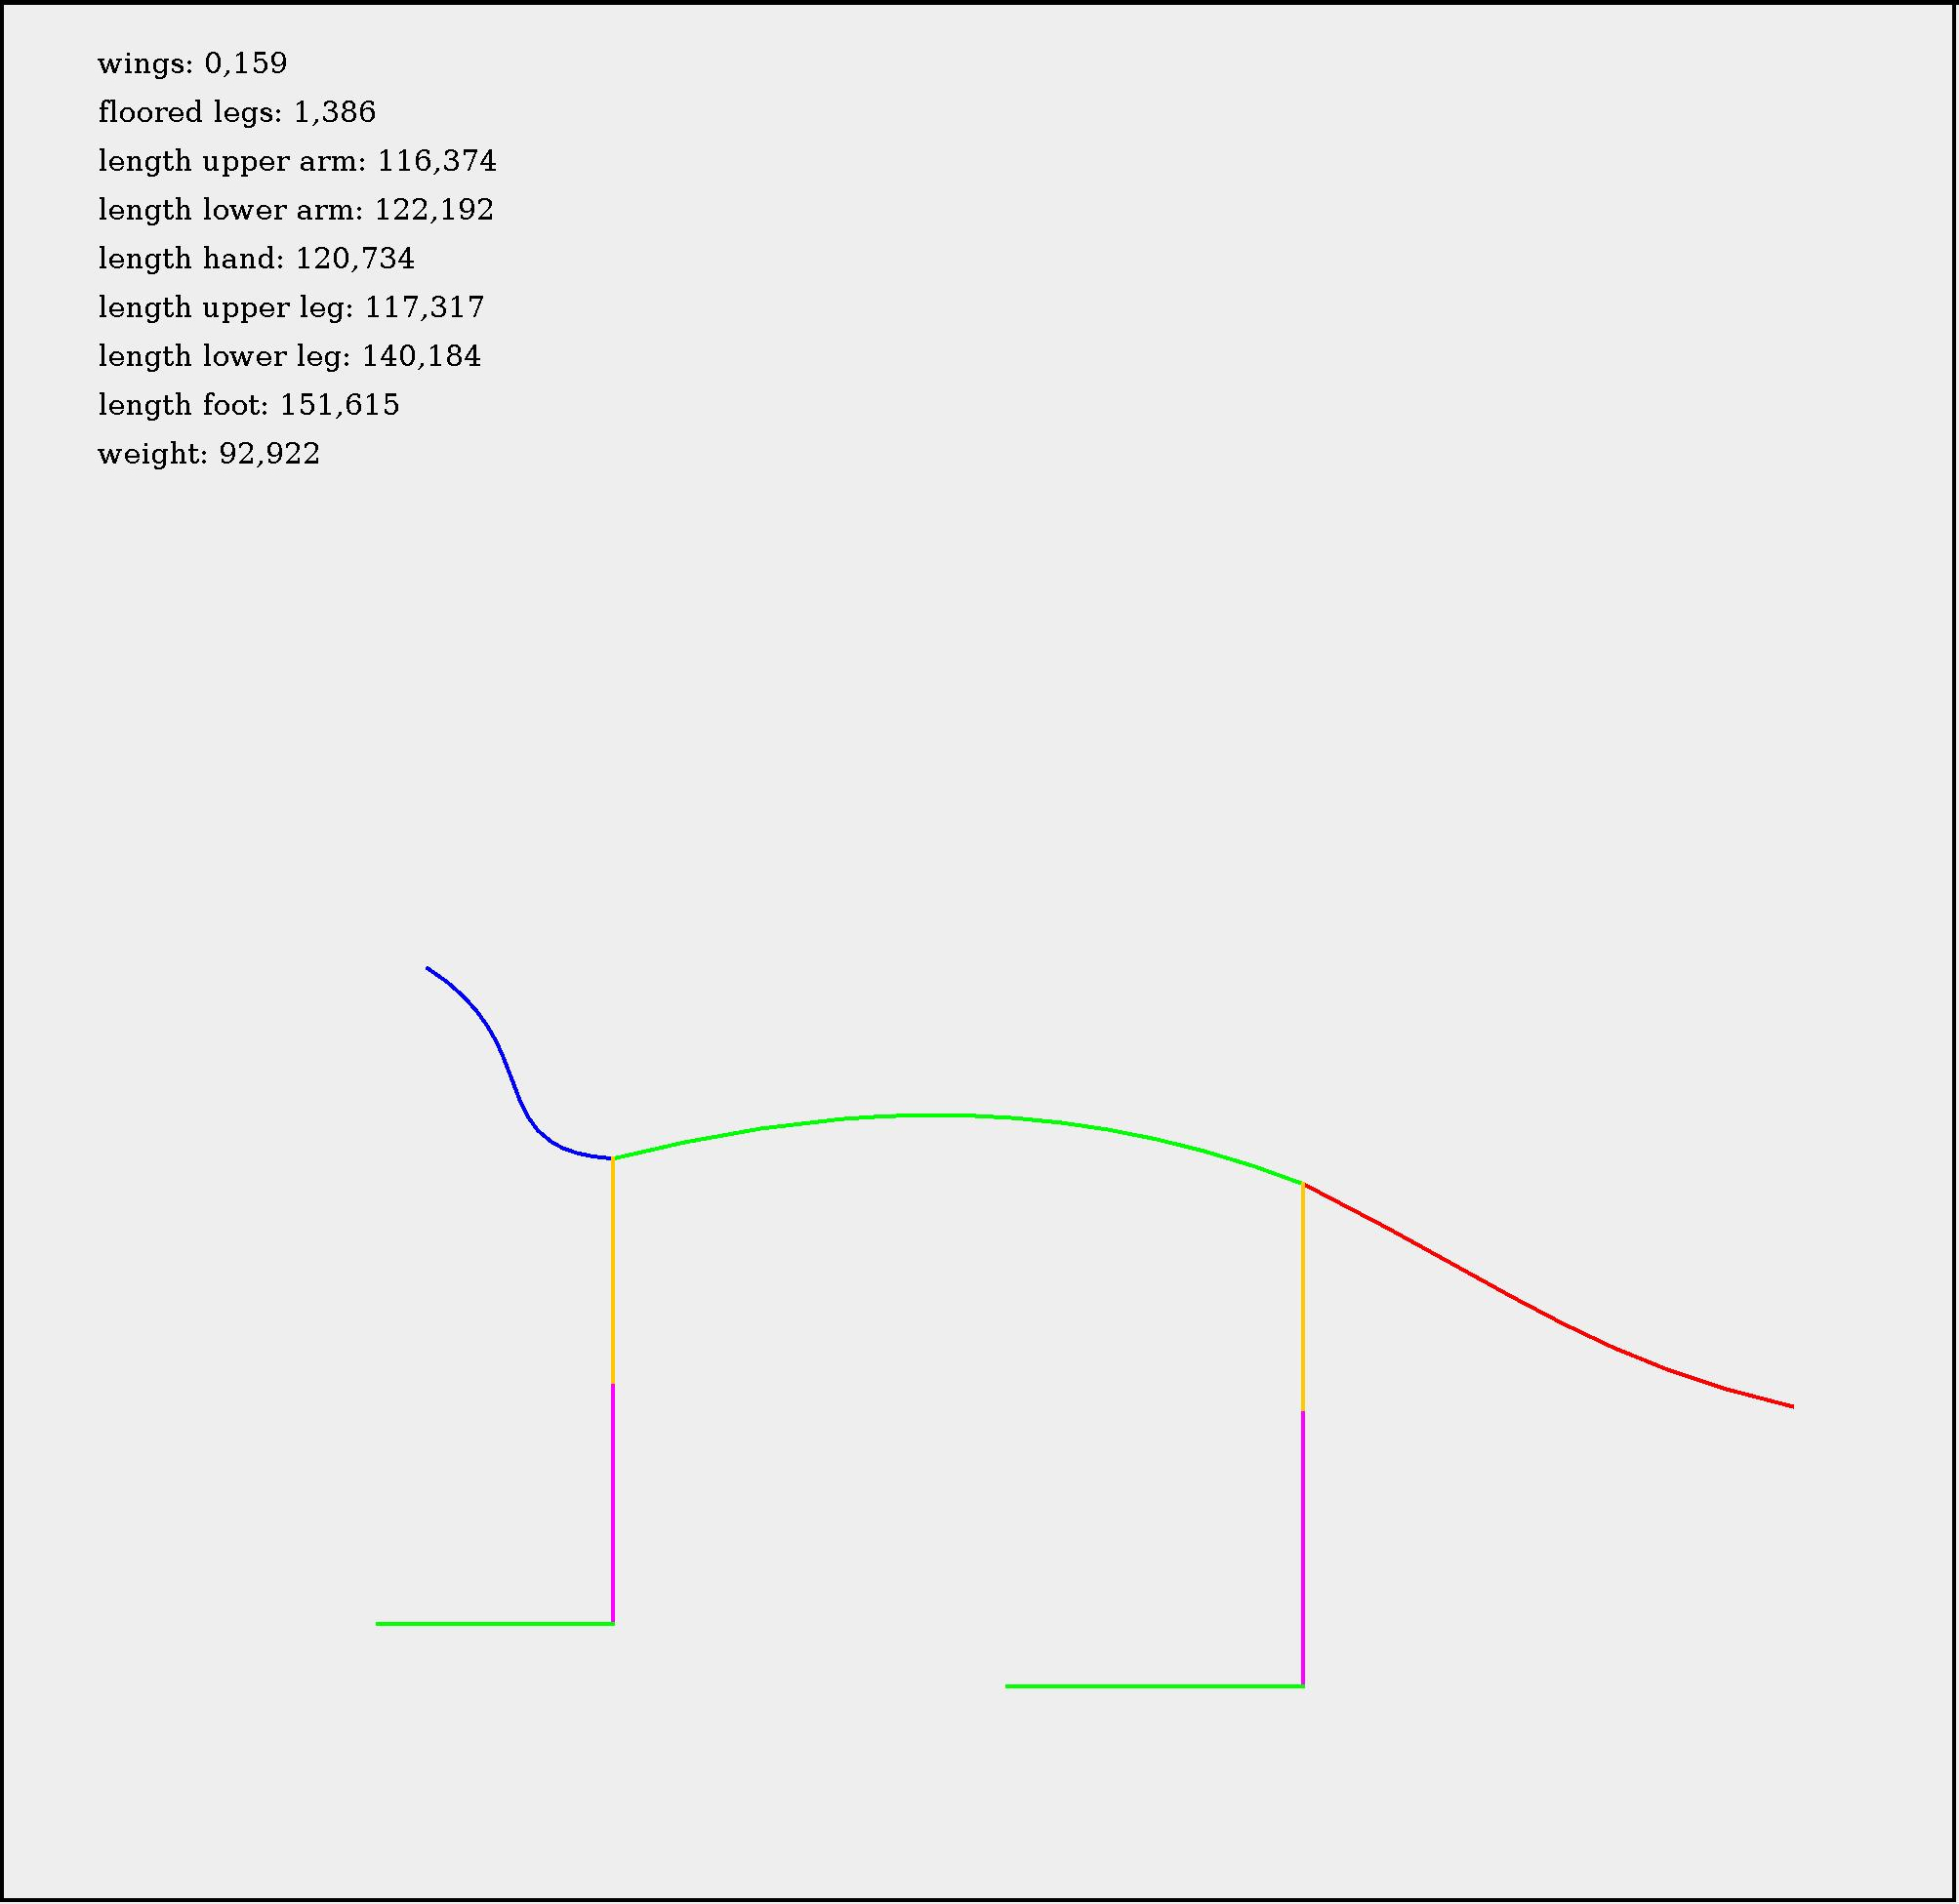
\includegraphics[width=0.7\textwidth]{../PCA/mean_log_weight.jpg}
  \caption{Visualisierung des Mittelwerts der Eingabedaten. Die Werte, die nicht visualisiert sind, sind folgende: ...}
  \label{mean_log_weight}
 \end{figure}
 
 Berachtet man die, in jeder Dimension auf das Intervall $[0, 1]$ skalierten Eingabedaten \todo{und alle anderen Anpassungen inkl. runterskalierte Flügel, Arme und Gewicht}, so hat der Klippschliefer den minimalen Abstand zum Mittelwert (siehe Abbildung \ref{klippschliefer_farbig}).
 
 Den maximalen Abstand hat die Schlange. Hier muss man aber dazu sagen, dass die Schlange der einzige Datenpunkt ohne Skelettbild ist. Das liegt daran, dass es keine seitlichen Abbildungen von ausgestreckten Schlangen gibt. Sie werden eigentlich immer gekrümmt dargestellt, da sonst das Bild sehr lang und schmal werden würde. Deshalb wurde für die Schlange eine horizontale Gerade knapp über dem unteren Bildrand gewählt, die den Rücken darstellen soll. Extremitäten und ersichtliche Punkte an denen der Rücken in Hals oder Schwanz übergeht gibt es ja keine.
 
 Der Punkt mit dem zweitgrößten Abstand zum Mittelwert ist das Känguru (siehe Abbildung \ref{kaenguru_farbig}).
 
 \begin{figure}
  \subfloat[Klippschliefer]{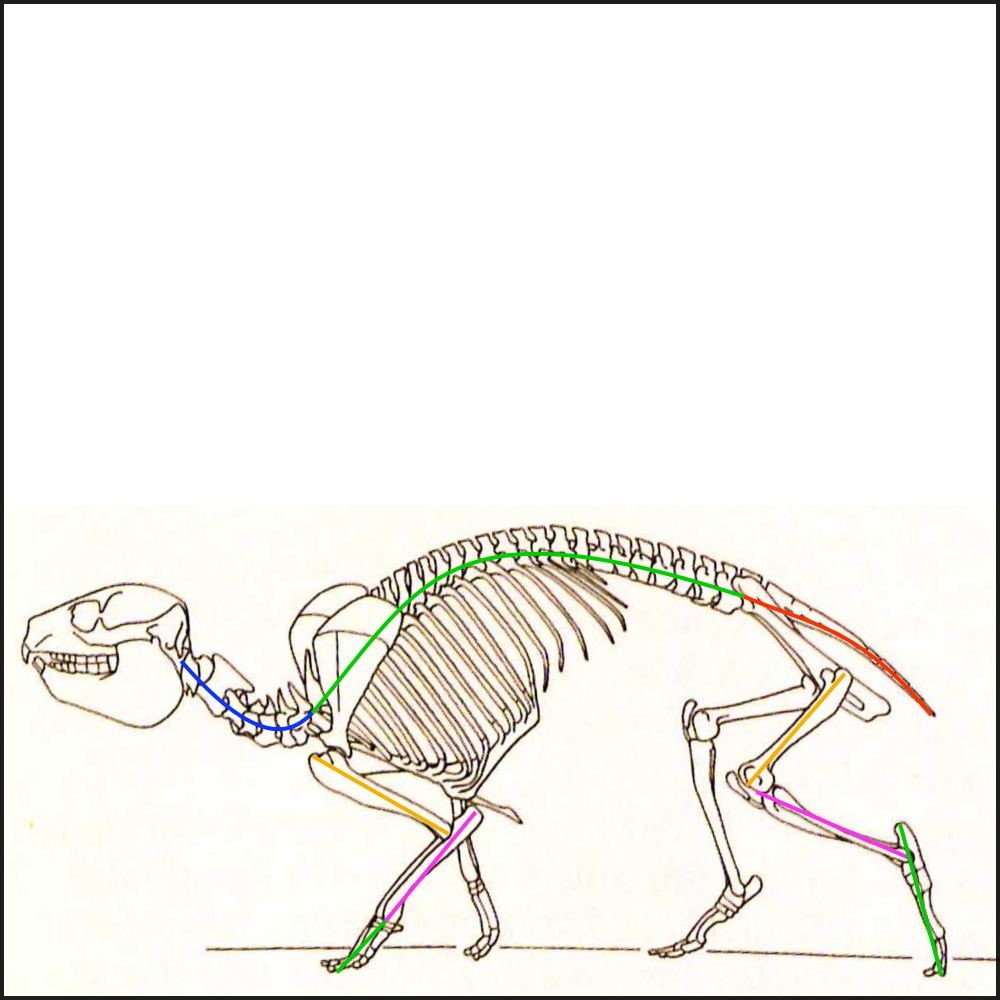
\includegraphics[width=0.5\textwidth]{../PCA/Skelettbilder/Klippschliefer_farbig.png} \label{klippschliefer_farbig}}
  \qquad
  \subfloat[Känguru]{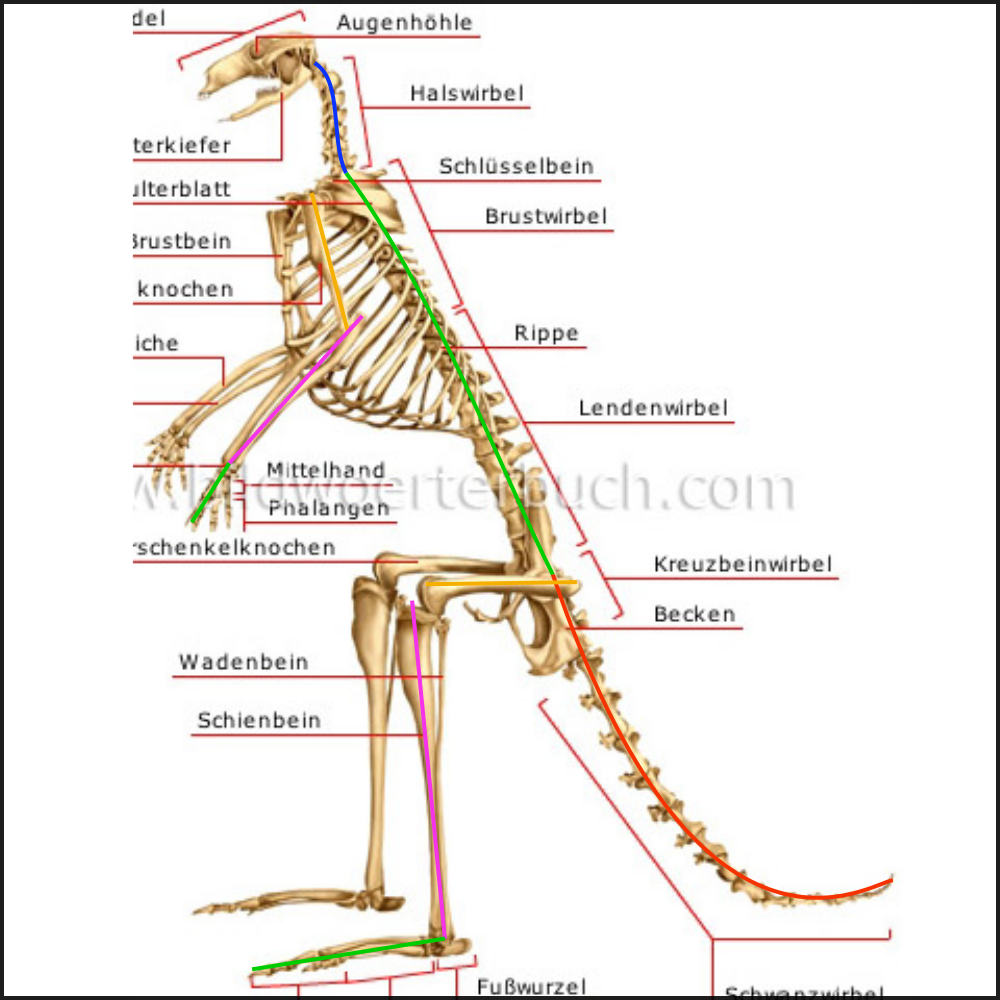
\includegraphics[width=0.5\textwidth]{../PCA/Skelettbilder/Kaenguru_farbig.png}\label{kaenguru_farbig}}
  
  \caption{Annotierte Bild des Skeletts eines Klippschliefers (a) und eines Kängurus(b). Zusätzlich wurde zum Klippschliefer erhoben:
  Tierklasse: Säugetier, keine Flügel, Anzahl Beine mit Bodenkontakt: $4$, ungefähres Gewicht: $4$kg; und zum Känguru: Tierklasse: Säugetier, keine Flügel, Anzahl Beine mit Bodenkontakt: $2$, ungefähres Gewicht: $50$kg.}
 \end{figure}

 
 Eine Vorraussetzung der PCA ist, dass die Eingabedaten in jeder Dimension normalverteilt sind. Es gibt die beiden Merkmale \emph{Flügel} und \emph{Beine mit Bodenkontakt}, die offensichtlich nicht normalverteilt sind, da sie diskret nur ein \bzw zwei Werte annehmen können. Hierzu weiter unten mehr. Die anderen Dimensionen wurden mithilfe eines Quantil-Quantil-Diagramms mit der Normalverteilung verglichen. \todo{QQ Diagramme erklären, negative Werte sind ganz normal, da inverse CDF bei einem Mittelwert von 0 bei Werten < 0.5 negativ ist.}
 Die Diagramm zeigen, dass die Dimensionen alle mehr oder weniger normalverteilt sind (siehe Abbildungen \ref{qqdiagram_examples} und im Anhang Abbildungen \ref{qq_diagrams_spine} und \ref{qq_diagrams_rest}).
 Für das Merkmal \emph{Gewicht} gilt dies aber nur, da es logarithmisch in die PCA eingeht. Die Verteilung der originalen Gewichte weicht sehr deutlich von einer Normalverteilung ab (siehe Abbildungen \ref{qqdiagrams_weight}).
 Verwendet man das lineare Gewicht als Eingabe für die PCA, treten dadurch bei der Kombination von zufälligen Werten für die Eigenvektoren schnell Gewichte kleiner null auf. Dies wird bei einer logarithmischen Skala vermieden.
 Welcher Logarithmus zur Umrechnung der Daten verwendet wird schlägt sich nur als linearer Faktor nieder. Da hier wiederum nicht ersichtlich ist welche Skalierung am besten wäre, wurde hier der Zehnerlogarithmus verwendet.
 
 \begin{figure}
  \subfloat[x-Wert der $3$. Koordinate des Halses]{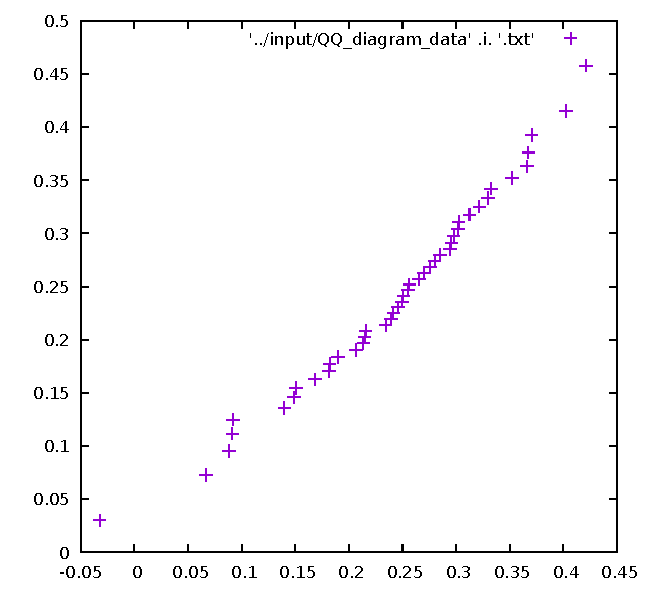
\includegraphics[width=0.3\textwidth]{../PCA/gnuplot/results_qq_diagrams/QQ_diagram4.pdf}}
  \qquad
  \subfloat[Länge der Hand]{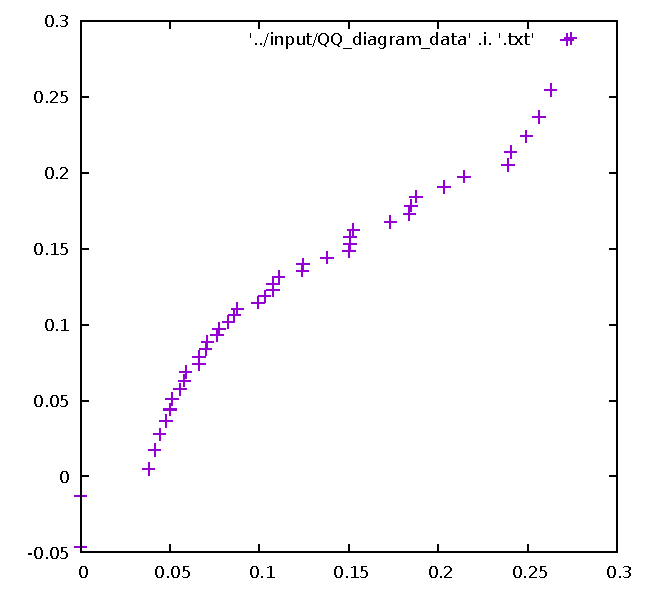
\includegraphics[width=0.3\textwidth]{../PCA/gnuplot/results_qq_diagrams/QQ_diagram24.pdf}}
  \qquad
  \subfloat[Länge des Oberschenkels]{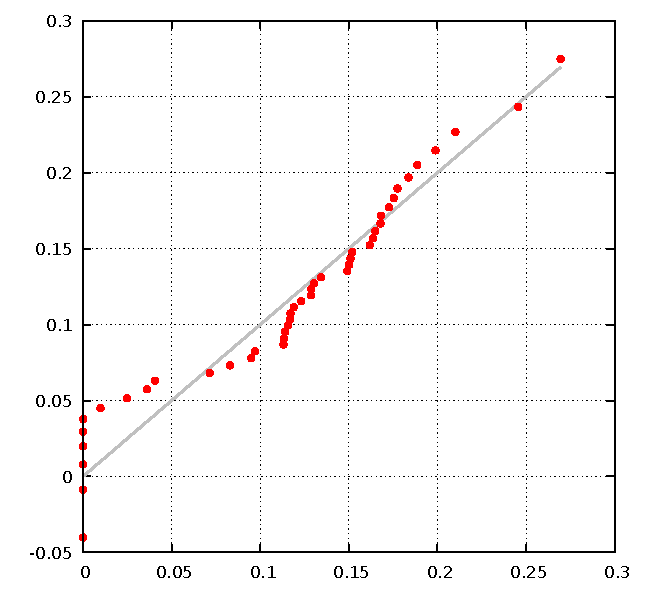
\includegraphics[width=0.3\textwidth]{../PCA/gnuplot/results_qq_diagrams/QQ_diagram25.pdf}}
  
  \caption{Beispielhaft ausgewählte Quantil-Quantil-Diagramme von drei Eingabedimensionen. (a) ist weicht nicht stark von der Normalverteilung ab, (b) und (c) hingegen schon mehr.}
  \label{qqdiagram_examples}
 \end{figure}
 
\begin{figure}
  \subfloat[Gewicht linear]{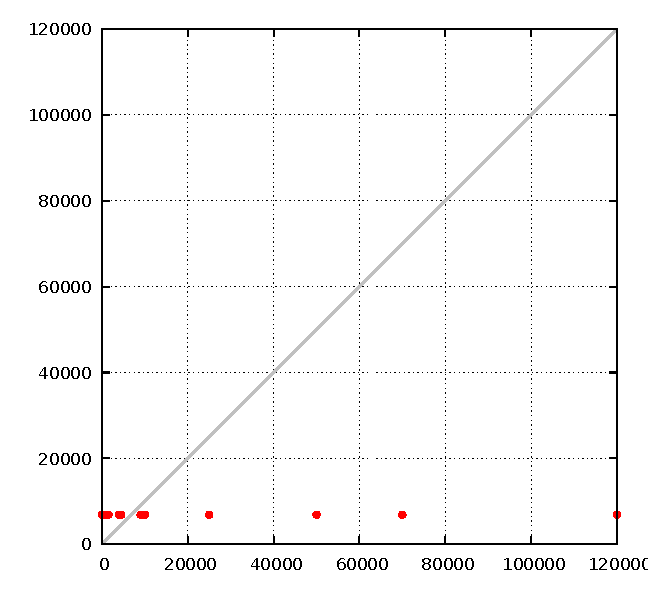
\includegraphics[width=0.3\textwidth]{../PCA/gnuplot/results_qq_diagrams/QQ_diagram_linear_weight.pdf}}
  \qquad
  \subfloat[Gewicht linear (Ausschnitt)]{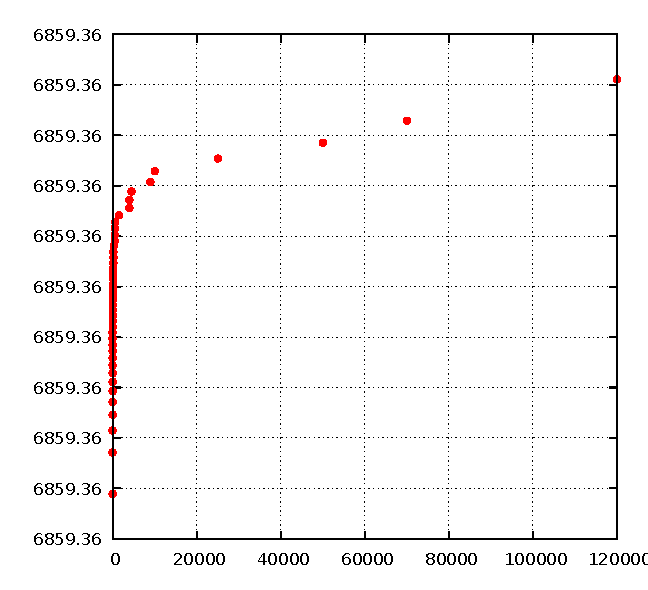
\includegraphics[width=0.3\textwidth]{../PCA/gnuplot/results_qq_diagrams/QQ_diagram_linear_weight_without_diagonal.pdf}}
  \qquad
  \subfloat[Gewicht logarithmisch]{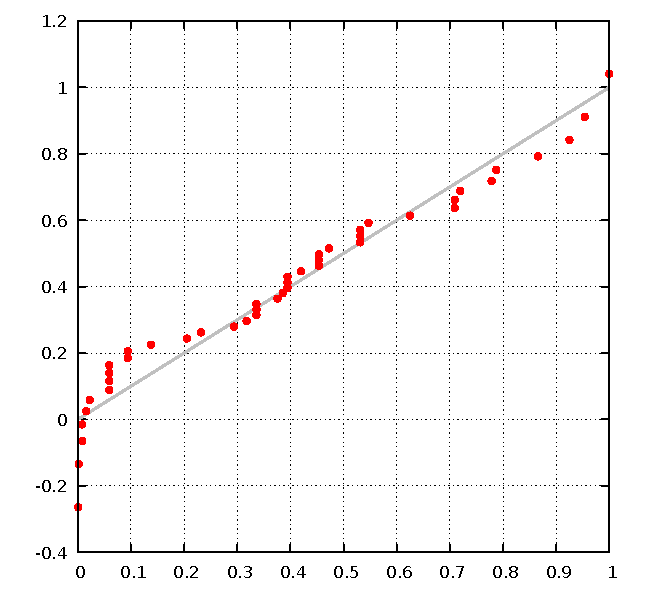
\includegraphics[width=0.3\textwidth]{../PCA/gnuplot/results_qq_diagrams/QQ_diagram28.pdf}}
  
  \caption{ Quantil-Quantil-Diagramme des Gewichts, einmal linear (a,b) und einmal mit logarithmischer Skala (b)}
  \label{qqdiagrams_weight}
 \end{figure}

 
 
 Im Folgenden werden die drei diskreten Merkmale \emph{Tierklasse}, \emph{Anzahl Beine mit Bodenkontakt} und \emph{vorhandene Flügel} genauer betrachtet.
 
 In Abbildung \ref{projections12} ist jeweils die Projektion der Daten auf die ersten beiden Eigenvektoren zu sehen. Klar zu erkennen ist, dass die Tiere mit Flügeln ein Cluster bilden. Betrachtet man die Daten annotiert mit der Tierklasse, so ebenfalls ein Cluster zu erkennen, das der Vögel. Das liegt daran, dass in den erhobenen Daten genau diejenigen Beispiele Flügel haben, die auch Vögel sind. Die restlichen Tierklassen hingegen bilden keine Cluster.
 Die Anzahl der Beine wiederum scheint ein gutes Unterschiedungsmerkmal zu sein. Hier sieht man wieder das Cluster der Vögel (in blau) mit vier Punkten zusätzlich, nämlich dem Känguru, dem Tyrannosaurus Rex, dem Seehund und der Ohrenrobbe. Und auch die anderen Gruppen bilden Cluster.
 
 
 \begin{figure}
  \subfloat[Flügel]{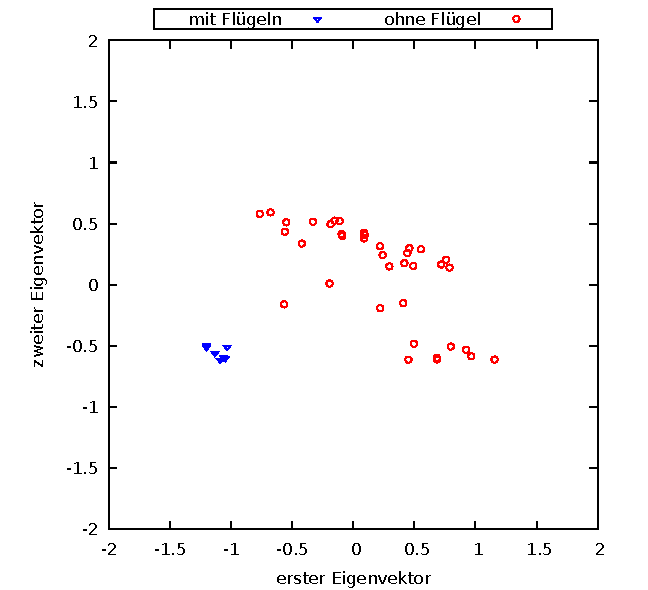
\includegraphics[width=0.3\textwidth]{../PCA/gnuplot_log_weight/results_with_wing_tag/projection_eigenvectors12.pdf}}
  \qquad
  \subfloat[Anzahl Beine mit Bodenkontakt]{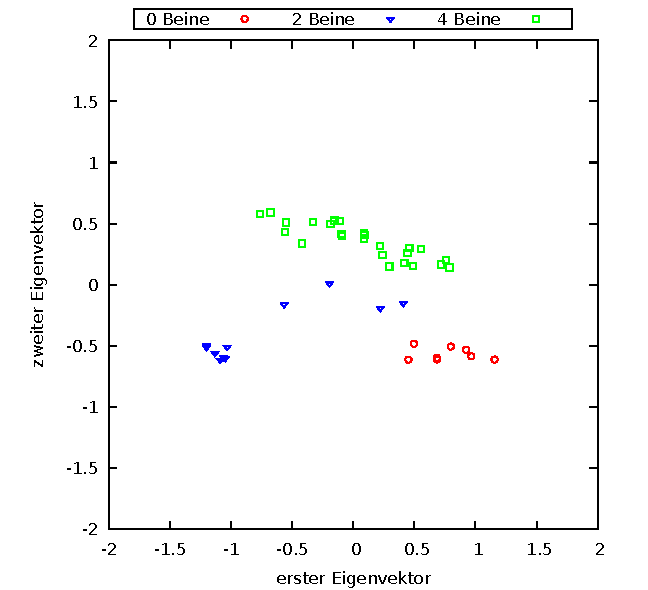
\includegraphics[width=0.3\textwidth]{../PCA/gnuplot_log_weight/results_with_leg_tag/projection_eigenvectors12.pdf}}
  \qquad
  \subfloat[Tierklasse]{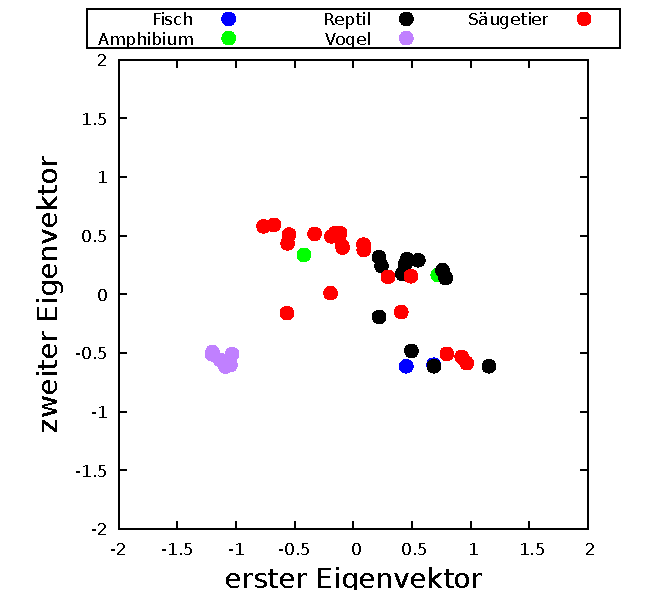
\includegraphics[width=0.3\textwidth]{../PCA/gnuplot_log_weight/results_with_animal_class_tag/projection_eigenvectors12.pdf}}
  
  \caption{Projektion der Eingabdaten auf die Ebene, die durch den ersten und zweiten Eigenvektor aufgespannt wird. Markiert sind jeweils verschiedene Merkmale der Punkte.}
  \label{projections12}
 \end{figure}
 
 Skaliert man Flügel und Beine um Faktor $1000$ kleiner, so verschwinden die Cluster (siehe Abbildung ...) \todo{Skalierung Beschreiben (auch schon in den vorherigen Abschnitten), Flügel, Beine und Gewicht mit 100 runterskaliert, damit sie nicht mehr in den ersten paar Eigenvektoren als große Werte vorkommen. Jetzt sind es meistens die kleinsten Werte. Soll keine Benutzereingabe sein, mehr Metadaten.}
 

 %- - - - - - - - - - - - - - - - - -
 \section{Analyse der PCA-Ergebnisse}
 \label{section_pca_result_analysis}
 
 Von $29$ Eingabedimensionen gibt es auch $29$ Eigenvektoren mit Eigenwerten größer $0$. Der kleinste hat einen Wert von $0,000024$. Von den Eigenwerten sind $7$ größer als $0,01$. Leider reichen diese $7$ Dimensionen aber noch nicht aus, um die Eingabedaten hinreichend anzunähern. Bei manchen Tieren funktioniert das ganz gut (siehe Archaeopteryx, Abbildung \ref{archaeopteryx}), bei anderen aber eher schlechter (siehe Frosch, Abbildung \ref{frosch}). Die Daten konnten somit von der PCA nicht besonders gut komprimiert werden. Trotzdem sind die berechneten Eigenvektoren hilfreich für die (Weiter-)Entwicklung des Algorithmus. \todo{wenn Algo weiterentwickelt, beschreiben}
 
 \begin{figure}
  \centering
  \subfloat[Rekonstruktion]{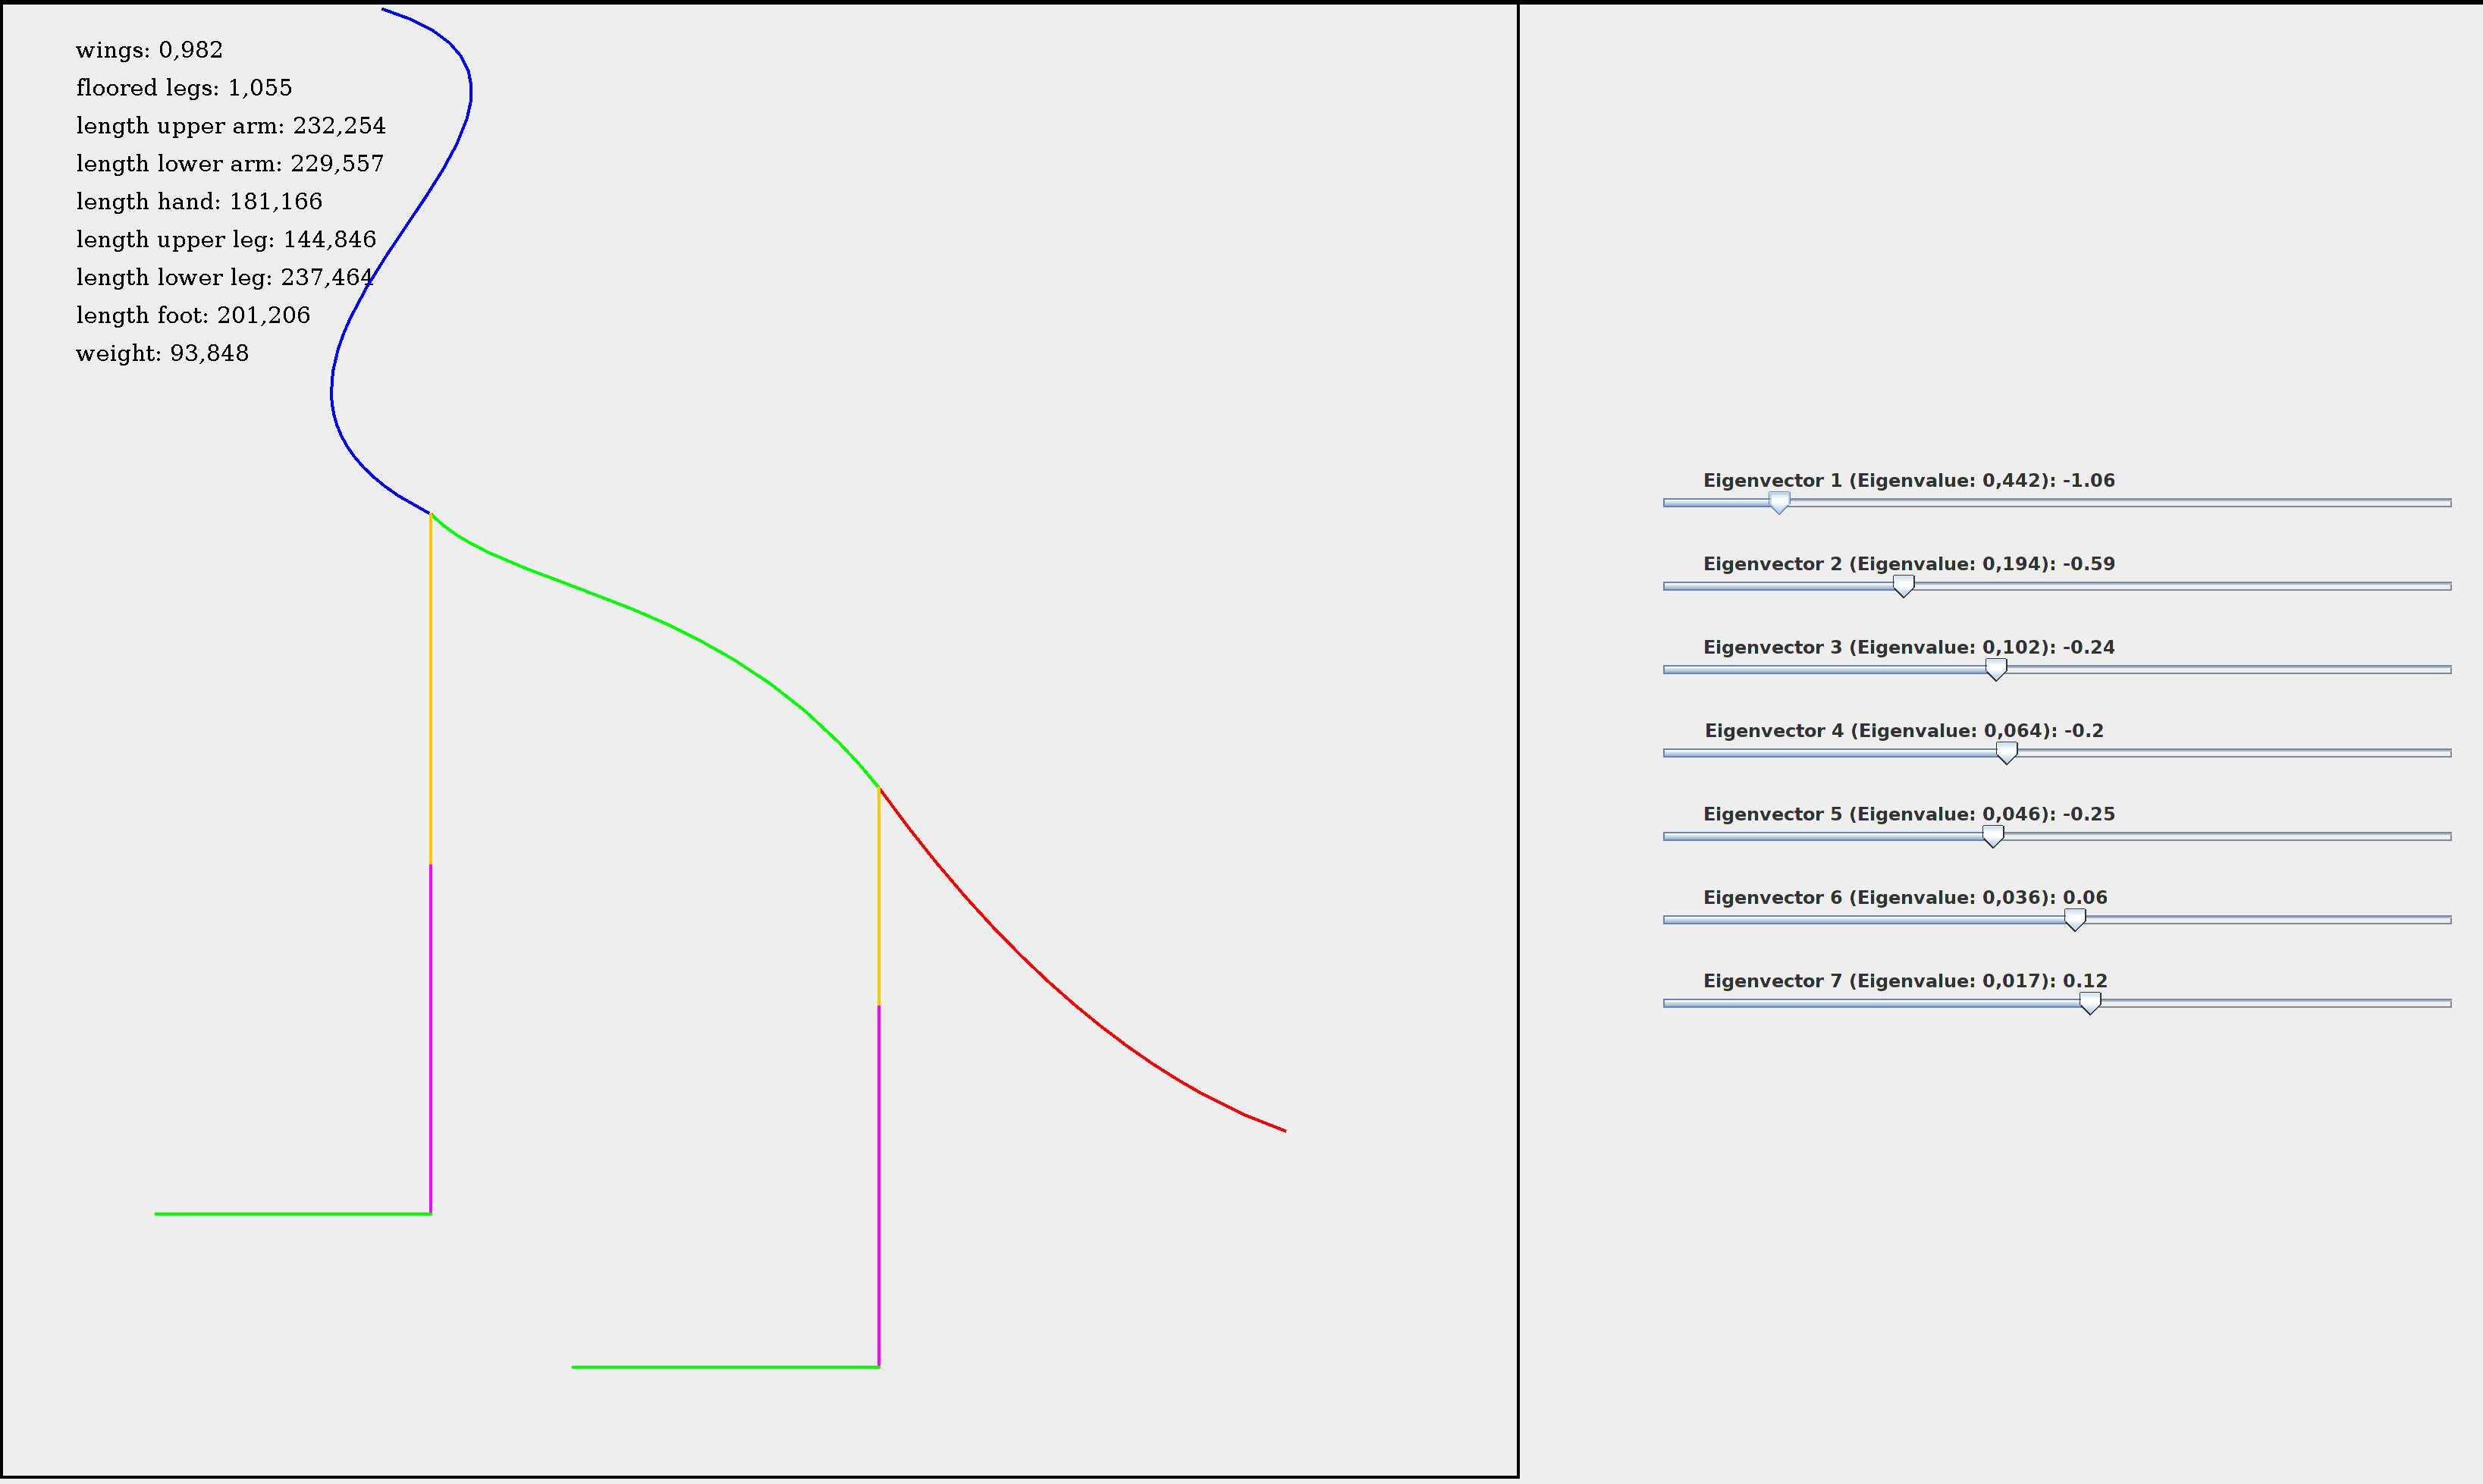
\includegraphics[width=\textwidth]{../PCA/animal_reconstructions_log_weight/Archaeopteryx.jpg}}
  \\
  \subfloat[Eingabebild]{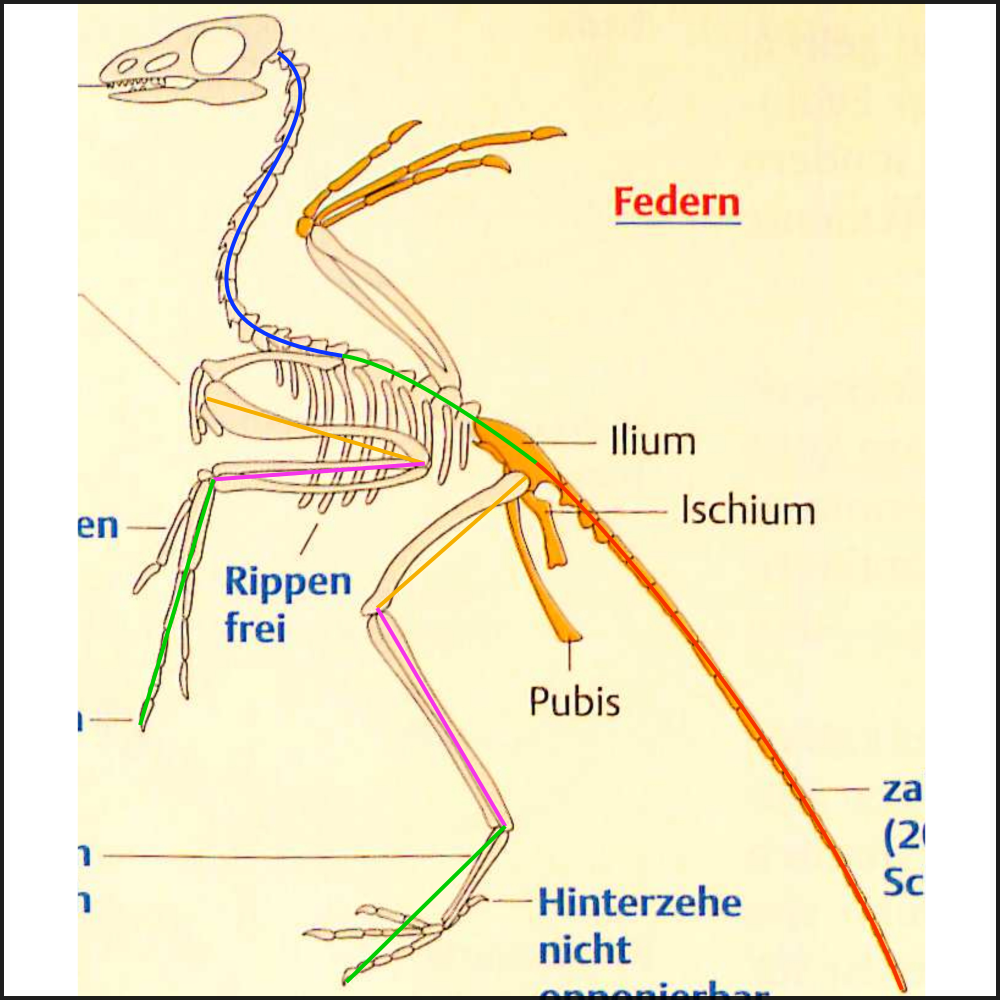
\includegraphics[width=0.5\textwidth]{../PCA/Skelettbilder/Archaeopteryx_farbig.png}}
  
  \caption{Archaeopteryx (a) Rekonstruktion aus den größten $7$ Eigenvektoren, (b) Eingabebild, zusätzlich erhobene Daten sind:
  Tierklasse: Vogel, Flügel, Paare von Beinen mit Bodenkontakt: $1$, ungefähres Gewicht: $1$kg}
  \label{archaeopteryx}
 \end{figure}
 
\begin{figure}
  \centering
  \subfloat[Rekonstruktion]{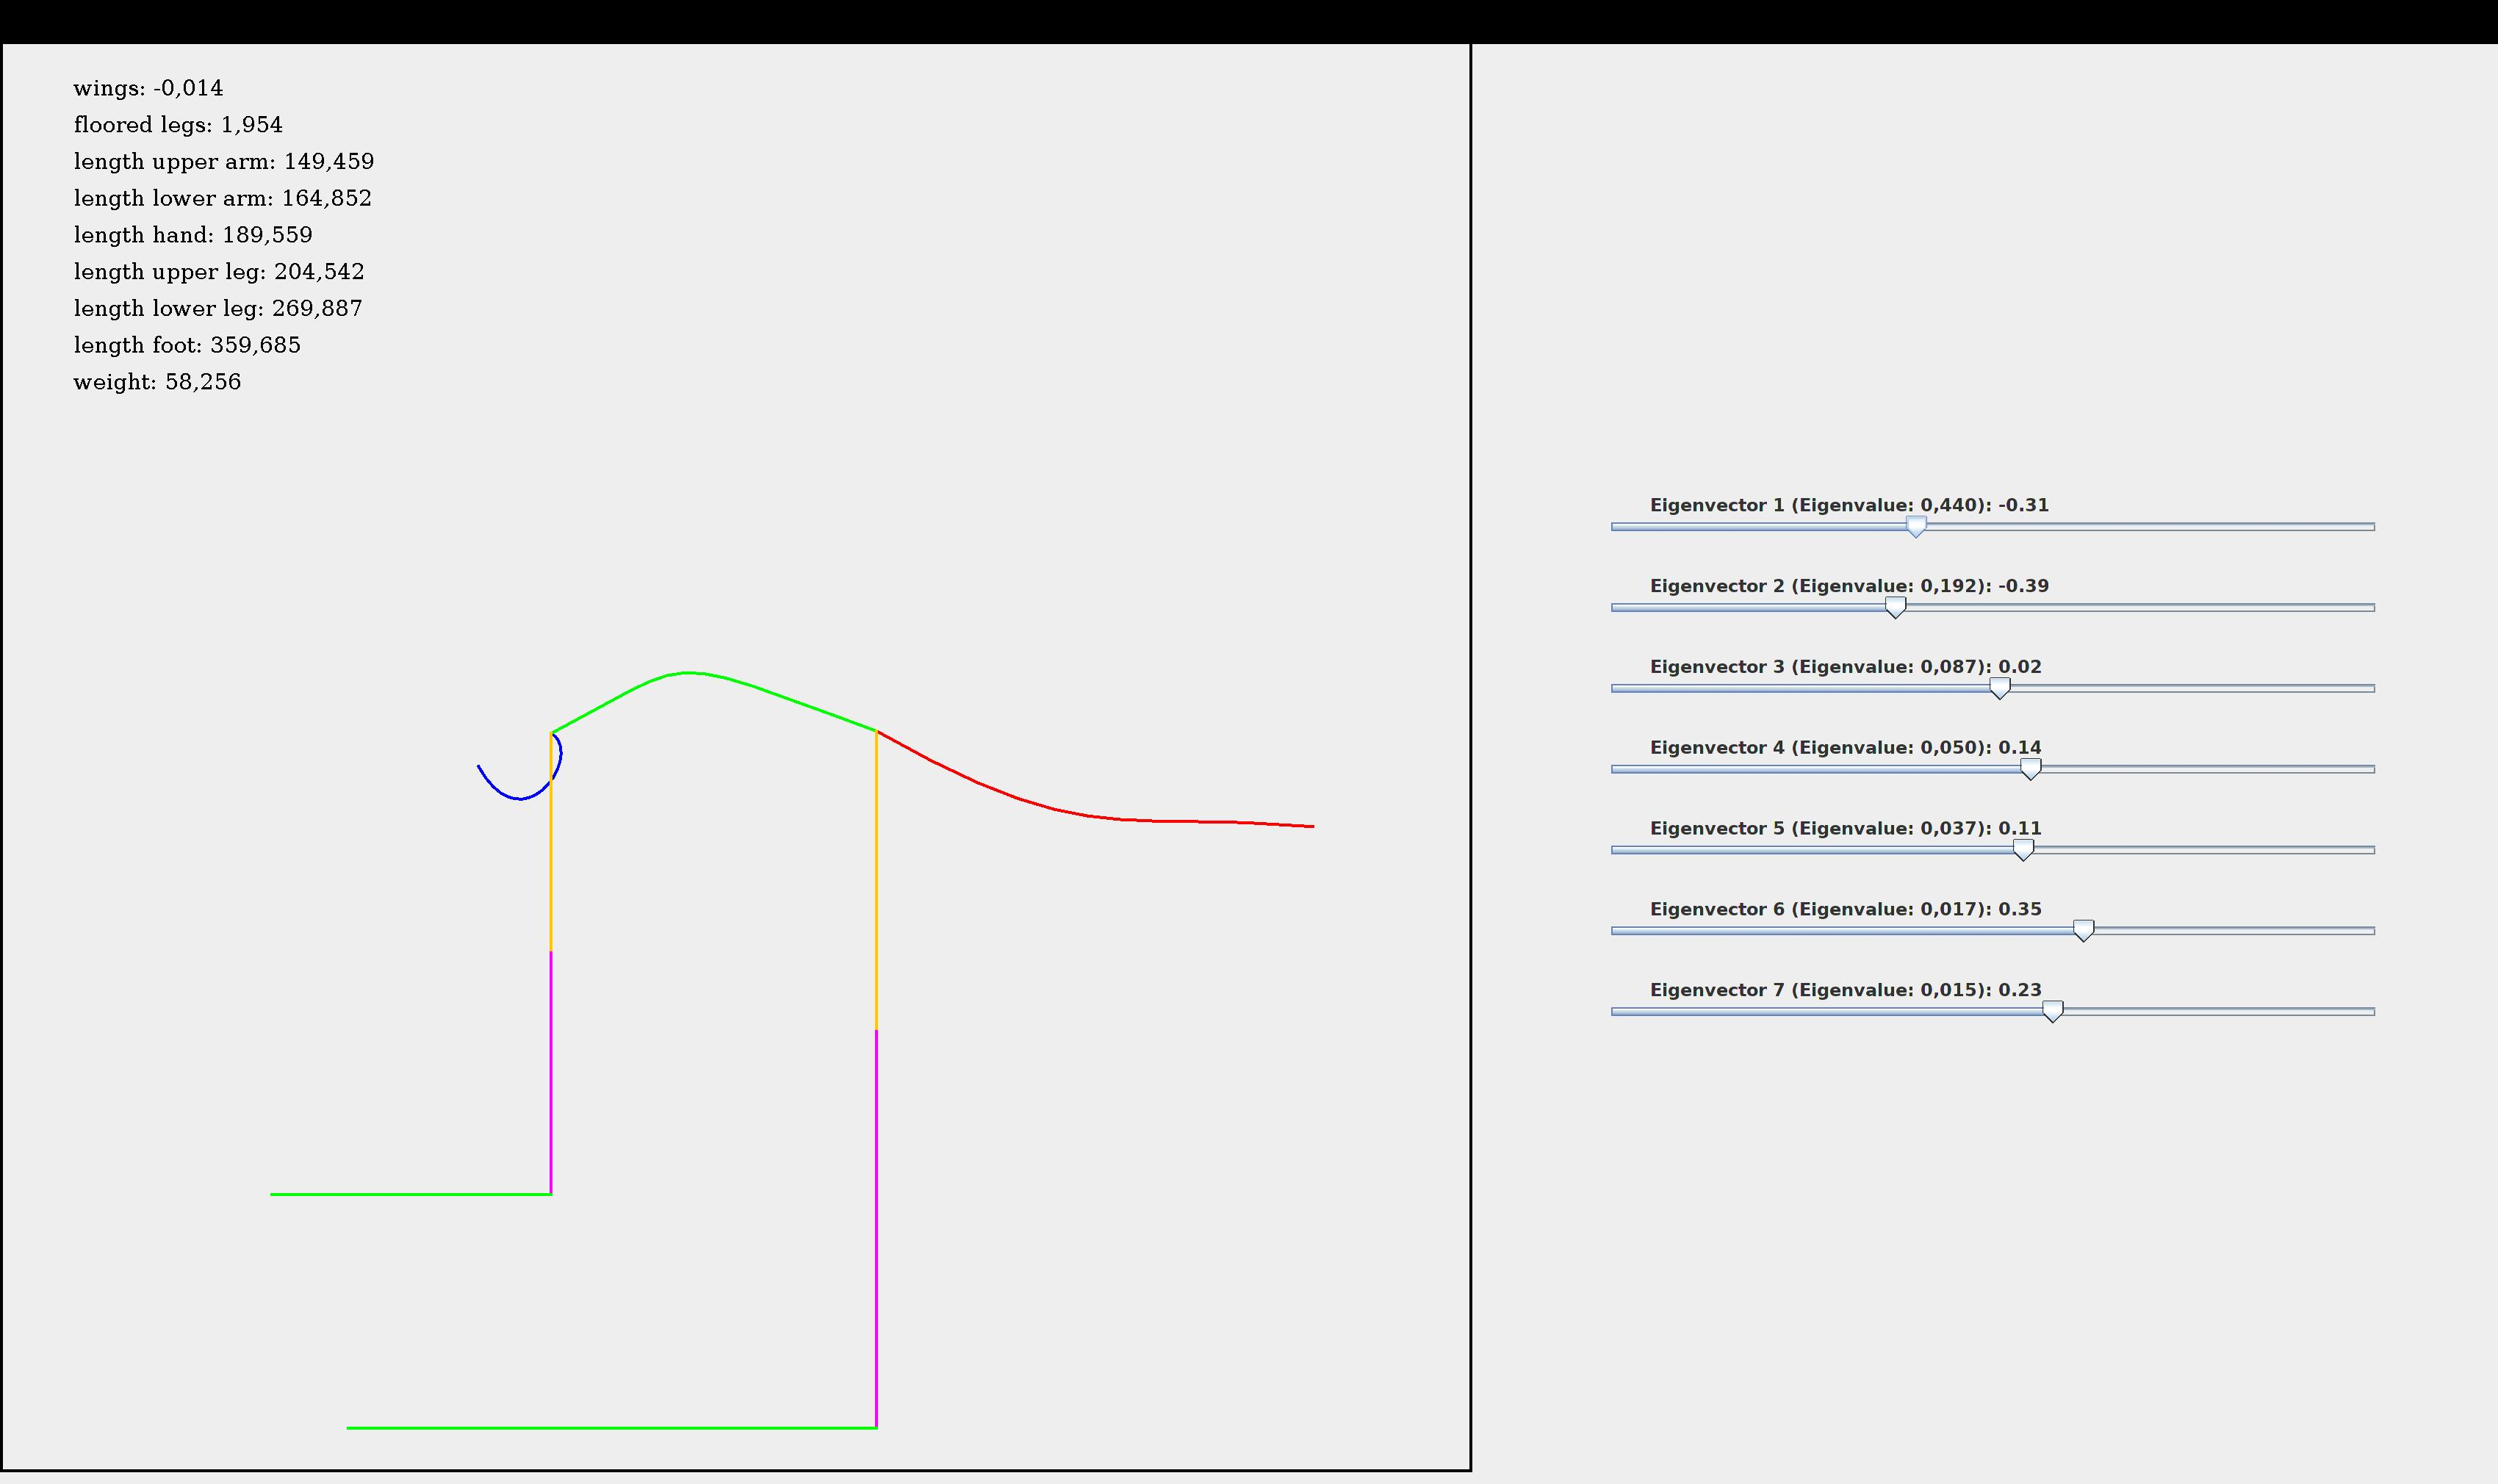
\includegraphics[width=\textwidth]{../PCA/animal_reconstructions_log_weight/Frosch.jpg}}
  \\
  \subfloat[Eingabebild]{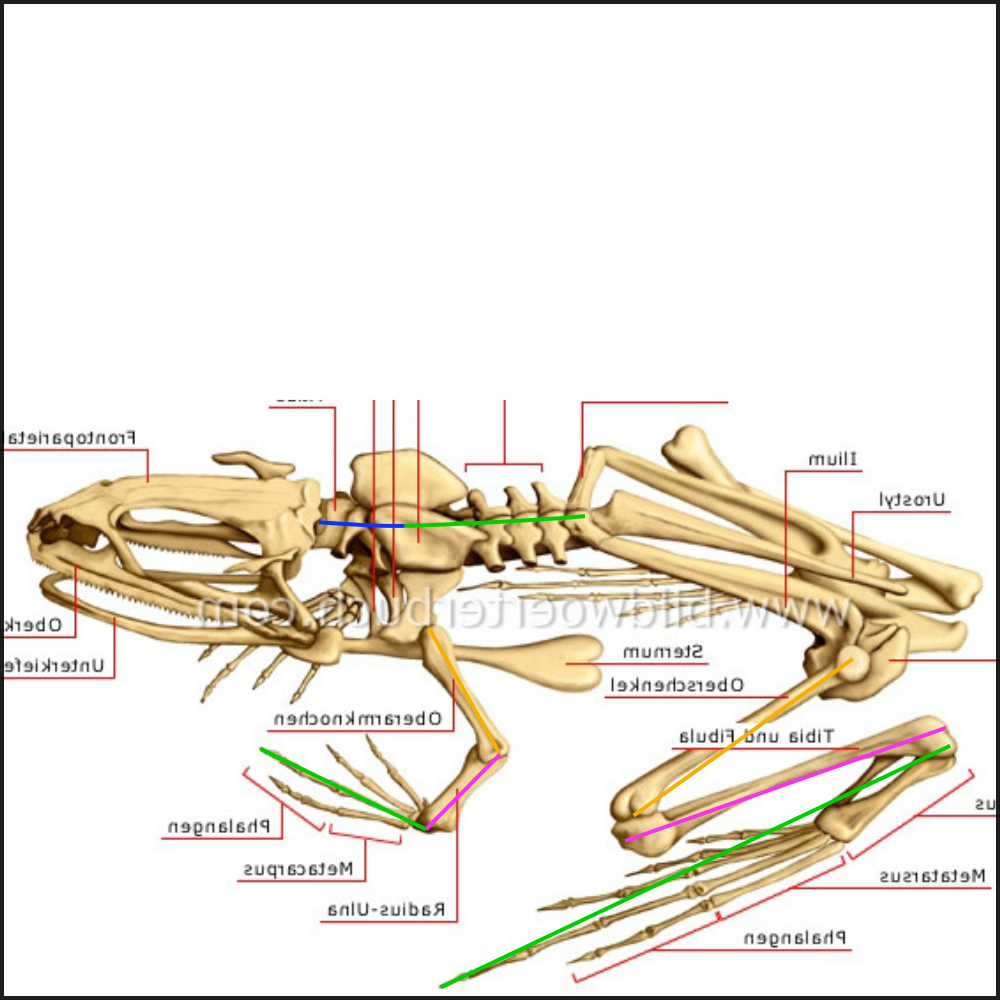
\includegraphics[width=0.5\textwidth]{../PCA/Skelettbilder/Frosch_farbig.png}}
  
  \caption{Frosch (a) Rekonstruktion aus den größten $7$ Eigenvektoren, (b) Eingabebild, zusätzlich erhobene Daten sind:
  Tierklasse: Amphib, keine Flügel, Paare von Beinen mit Bodenkontakt: $2$, ungefähres Gewicht: $0,01$kg}
  \label{frosch}
 \end{figure}
 

 In den Abbildungen, die die Eingabedaten im transformierten Koordinatensystem der PCA darstellen (Abbildung \ref{projections12}) ist gut zu erkennen, dass die Koordinatentransformation der PCA die Daten tatsächlich nach den Hauptachsen des mehrdimensionalen Ellipsoids, den die Datenpunkte bilden, ausrichtet.

 Bei allen Eingabedimension, außer der Position der Wirbelsäule, kann man sich die Frage stellen, ob sie nötig sind, oder ob sie eher die Ergebnisse der PCA verschlechtern. Es wurde ausprobiert verschiedene (Kombinationen von) Merkmalen wegzulassen. Die Ergebnisse unterscheiden sich nicht extrem von der PCA mit allen Daten. 
 
 Leider gibt es keine gute Möglichkeit die Qualität der Ergebnisse der PCA zu messen. Man könnte den Unterschied zwischen den Eingabedaten und den Rekonstruktionen aus den Linearkombinationen der Eigenvektoren mit den größten Eigenwerten messen. Aber das liefert, durch das Fehlen von verschiedenen Dimensionen kein einheitliches Maß.
 
 Da jede Dimension dem Algorithmus, der später Skelette generieren soll, helfen könnte, haben wir uns dafür entschieden alle Merkmale zu behalten.
 
 Außerdem gibt es die Möglichkeit die Eingabedaten in mehrere Mengen aufzuteilen und diese von verschiedenen Instanzen der PCA analysieren zu lassen. Hierbei gibt es zunächst das Problem, dass sich dann die Anzahl der Datenpunkte noch weiter reduziert, was die Ergebnisse nicht mehr repräsentativ macht.
 Ein Merkmal, das sich zur Unterteilung in Mengen anbieten würde, ist die Angabe ob das Tier Flügel hat oder nicht, da sich dadurch nur zwei Gruppen ergeben. Außerdem ist die Gruppe der Tiere mit Flügeln in den Eingabedaten klar als Cluster zu erkennen (siehe auch Abschnitt \ref{pca_input_analysis}). Tatsächlich liefert eine solche Aufteilung bessere Rekonstruktionen aus der größten Eigenvektoren, aber das liegt natürlich vor allem daran, dass die zu untersuchende Datenmenge, jeweils verkleinert wurde.
 
 Ein Problem dabei ist, dass dann keine Skelette mehr erzeugt werden können, die zwischen den beiden Gruppen liegen. Tatsächlich scheinen die Datenpunkte, die "`zwischen"' den Gruppen erzeugt werden, relativ sinnvoll auszusehen.
 Das wäre ein Argument dafür keine Aufteilung vorzunehmen. Dasselbe gilt für die Cluster, die durch die Aufteilung anhand der Anzahl der Beine mit Bodenkontakt entstehen.
 

